%!TEX encoding = UTF-8 Unicode
% $Id: Rapport.tex 39 2012-11-05 17:40:35Z Vincent.Plasse $
 
\documentclass[a4paper,11pt]{report}

%algorithme
\usepackage{amsmath}
\usepackage{amssymb}
\usepackage{algorithm2e}


\usepackage{comment} %Commentaire

\usepackage[pdftex, 	 
bookmarks = true, 	% Signets
bookmarksnumbered = true, 	% Signets numérotés
pdfpagemode = None, 	% Signets/vignettes fermé à l'ouverture
pdfstartview = FitH, 	% La page prend toute la largeur
pdfpagelayout = SinglePage, 	% Vue par page
colorlinks = true, 	% Liens en couleur
urlcolor = magenta, 	% Couleur des liens externes
pdfborder = {0 0 0} 	% Style de bordure : ici, pas de bordure
]{hyperref} 	% Utilisation de HyperTeX

\usepackage[citestyle=authoryear]{biblatex}
\addbibresource{Source.bib}
\usepackage{verbatim} 
\usepackage[utf8]{inputenc}
\usepackage[T1]{fontenc}
\usepackage[francais]{babel}
\usepackage{graphicx} %image
\graphicspath{{./IMG/}}
\usepackage{epstopdf}
\usepackage{epsfig}
\hypersetup{
	colorlinks,
	citecolor=red,
	linkcolor=black,
	urlcolor=blue}


%%%%%%%%%%%%%%%%%%%%%%%%%%%%%%%%%%%%%%%%%%%%%%%%%%%%%%%%%%%%%%%%% VARIABLES %%%%%%%%%%%%%%%%%%%%%%%%%%%%%%%%%%%%%%%%%%%%%%%%%%%%%%%%%%%%%%%%%%%%%%%%%%%
\newcommand{\Titre}{Project Research and developpement}
\newcommand{\Auteur}{Matéo Rémi & Vincent Plasse}
\newcommand{\HRule}{\rule{\linewidth}{0.5mm}}
\title{\Titre}
\author{\Auteur}
\date{\today}

\begin{document}

\begin{titlepage}%ta page de titre
%les deux logos en haut

\begin{center}
% Upper part of the page

\includegraphics[width=0.5\textwidth]{POLYTECH.jpg} \\[3cm]    

\textsc{\LARGE Polytech Nantes}\\[0.5cm]

\textsc{\Large Project Research and developement}\\[0.5cm]


% Title
\HRule \\[0.4cm]
{ \huge \bfseries DGtal Advance}\\[0.4cm]

\HRule \\[1.5cm]

% Author and supervisor
\begin{minipage}{0.4\textwidth}
\begin{flushleft} \large
\emph{Authors:}\\
Rémi \textsc{Matéo}\\
Vincent \textsc{Plasse}
\end{flushleft}
\end{minipage}
\begin{minipage}{0.4\textwidth}
\begin{flushright} \large
\emph{Supervisors:} \\
Nicolas \textsc{Normand}\\
Eric \textsc{Remy}
\end{flushright}
\end{minipage}
\\[3cm]

\includegraphics[width=0.5\textwidth]{irccyn_transparent.png} \\[2cm]    

% Bottom of the page
{\large \today}

\end{center}

\end{titlepage}
\newpage
\tableofcontents

\chapter{Introduction}
\chapter{Thanks}
\chapter{Requiered}
\subsection{Distance}

\subsection{Library compilation}
       In this project we used some library. there is two ways to use it.
       first you can use a static compilation which include what the programme need before the execution. The executable may be big but he is not fragile to library's update.
       The second way consist to link your application with the library it's called dynamic compilation. The executable is smaller than the other but he is more fragile to library's update.
       
\subsection{Template}
       Today many library are implemented with Template. with template that allows you to define a fonction for many type or class you have to used. And that's it the compilator will generate the function specific that you used in the application. That explain than the compilation will be more longer if you use template but the execution is faster.

\section{Boost}
In this part we will describe some particularity of boost to have a better knowledge about this library.
To understand this part you should at least have a basic knowledge about c++, especially pointer.
Boost is used by famous company like Nvidia, Adobe and Microsoft.
Boost is a rally of many libraries and algorythm.
We will now see some news evolution between the c-pointer and the new pointer.
for any further informations i refer to the official documentation written by \cite{boostdocumentation}.
If you have never heard something about Boost i recommand to you this book written by \cite{introductionboost}. %test

\subsection{Pointer}
\subsubsection{auto\_ptr}
std::auto\_ptr is standard pointer which can automatically call the delete that you should do with old pointer.\\
It's easy to manipulate this pointer because you can use the same syntax than the old thanks to operator surcharge.
Now with auto\_ptr you don't have to put delete to every catch to desallocate properly your object.


\noindent{\textbf{How does it work?}}\\
The auto\_ptr have only one ownership and when the life of the variable auto\_ptr is destroy the delete is automatically called.\\
Example :
\begin{verbatim}
#include <iostream>
#include <memory>

using namespace std;

class A{
public:
~A(){ cout << "A is destroy" << endl;}
};


int main()
{
auto_ptr<A> smart_ptr(new A());
return 0;
}//A is automaticaly delete because smart_ptr is destroy
\end{verbatim}




\noindent{\textbf{Warning}}\\
When you have multiple auto\_ptr on the same object. the last is the ownership. \\
Example of typical error: \\
\begin{verbatim}
int main()
{
auto_ptr<A> smart_ptr(new A());
cout << smart_ptr->toString() << endl;
if(true)
{
        auto_ptr<A> smart_ptrB(smart_ptr);

}// here A is destroy

cout << smart_ptr->toString() << endl;//A not exist

return 0;
}
\end{verbatim}


\subsubsection{Scoped\_ptr}
Scoped\_ptr are a different smart\_ptr. It's special because you don't have transfert ownership and it isn't copyable.
So you just have to use it for temporary object.
So we can use it to say the object that you use is temporaire, it can be destroy at any time.



\subsubsection{Shared\_ptr}
Shared\_ptr is a smart\_ptr really interesting because that doesn't work like auto\_ptr.
It's an object which have a counter of references. What does that means? %citer la documentation
when shared\_ptr are destroy is simply check if that was the last or not, if it's he call the destructor for the ressources.
Moreover that pointer is thread safe we will see more informations about thread below. \\

%faire un schéma avec les references
\begin{figure}
	\center
	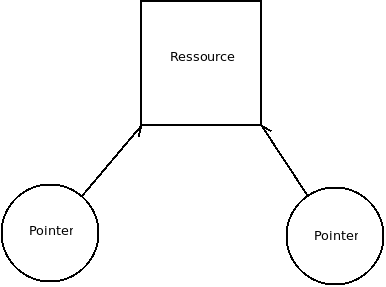
\includegraphics[width=0.75\textwidth]{Shared_ptr.png}
	\caption{Shared\_ptr scheme}
\end{figure}
\newpage
Example :\\
You can have multiple shared\_ptr on one ressource when all of them are destroy the ressources are destroy. There is nothing about ownership.
\begin{verbatim}
int main()
{
boost::shared_ptr<A> smart_ptr(new A());//1
cout << smart_ptr->toString() << endl;
if(true)
{
	boost::shared_ptr<A> smart_ptrB(smart_ptr);//2
	cout << smart_ptrB.use_count() << endl;

}
cout << smart_ptr.use_count() << endl;//1
cout << smart_ptr->toString() << endl;

return 0;
}//0 A is destroy 
\end{verbatim}

\subsubsection{Weak\_ptr}
This pointer exist to complete the shared\_ptr.
the shared pointer can create a weak\_ptr to his ressources which can cancel the delete.
This weak pointer can be create from lock methode or using shared\_ptr.
That allows you do transmit a pointer to a ressources even if the old shared\_ptr is destroy.


\subsection{Thread}


With boost you can initialize a thread and manage to wait the end of the process in your principal process with the method join.
You also can manage and create thread with included boost::thread in you application or lib.
You also still use mutex moreover the code than you produce is portable (thread part).
If you already know pthread you will be able to use the boost::thread the same name for the methode.

\begin{figure}
	\center
	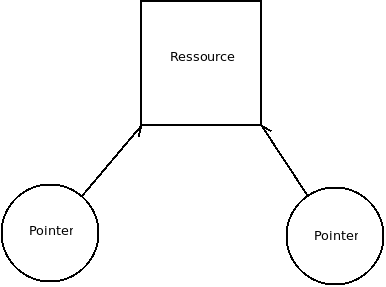
\includegraphics[width=0.75\textwidth]{Shared_ptr.png}
	\caption{Shared\_ptr scheme}
\end{figure}
Here it's a nice scheme about thread, if you have some difficulties I recommend to you to read this article.


\section{DGtal}
\subsection{Presentation}
\subsubsection{What is DGtal}

DGtal is a open Source library for Discrete Geometry Programming.
The library is accessible by anyone and it's a good library for demonstration.
That is using also to compare different algorithme with performance as a consequently you can use it as indicator.

\subsubsection{How DGtal works}
The library is divided in package.
Here it's some general package :
	-Mathematical Package(polynomial)
	-IO Package (to export/import and visualize with different format)
	-Image Package (Linear vector)
	-Geometry Package (model and algorithms)
	-Topology package
	-Kernel Package
	-Arithmetic Package

if you want more informations about it, I suggest you to see the David CoeurJolly Presentation \cite{davidcoeurjollypresentation}.

\subsubsection{How DGtal is Develloped}
The documentation of DGtal is implemented with Doxygen. \\
The team of DGtal use github for the project so you can access in mode read only to all the new feature. \\
You have three repository : \\
	-DGtal (main Library) \\
	-DGtalTools (Command line tools for analyzer etc) \\
	-DGtalScripts (script for developpers)

\subsubsection{What will use in DGtal}
We will work in Geometry packages for this project more precisely in volumetric nd package. \\
%http://libdgtal.org/doc/stable/moduleVolumetric.html
First of all we have to define our Metric with the class CSeparateMetric and then after that we will use DT or just make our class to it. \\
%http://libdgtal.org/doc/stable/structDGtal_1_1CSeparableMetric.html
We will probably work in the first time with Z2i namespace because this is the standard set of types for 2D imagery. \\
%http://libdgtal.org/doc/stable/namespaceDGtal_1_1Z2i.html#aca523bebdae58eb19385aaefffff8bc5

Finally to checks our result we will use output image to save our result and export in some format with the package I/O. We can also display it with Board2D from I/O Package. \\
%http://libdgtal.org/doc/stable/classDGtal_1_1DistanceTransformation.html#a01875821fcfd395cee6b2282275d84af
%http://libdgtal.org/doc/stable/dgtal_dgtalboard.html

For any further informations I recommend to read the official documentation of DGtal \cite{dgtaldocumentation}.

\subsubsection{Technical View}
To have a better knowledge about DGtal you have to create a github account.
That will allows you to fork the project to know the organisation about source module.
As you can see they use CMake to test their module and compil. they also have a strong organisation
they separate inline implementation than one and more line.
.ih for inline
.cpp for implementation
.h for description.
You also can see that you have many comments with the syntax of Doxygen.


\chapter{State of the art}

\section{Abstract}
\chapter{Solution}
In this part we will explain what algorithm we have to implement and how it's works.
A picture is composed a set of point which point can be pixel or something else it does'nt matter.
We have a mask which we will used for the propagation.
With this propagation we will be able to determine the minimum cost to access from outside of the picture to the point.
We need to have two propagation to get a map of correct distance for each point. In fact that depends about the mask than you want to used. \\

\subsection{Algorithm Distance} 
\begin{algorithm}[H]


\KwData{ \\ $X$ set of point \\ $M$ neighborhood with the mask \\ $cost$ minimal cost of the way}
\KwResult{Number distance}

\ForAll{$point$ in $X$}
{
	\eIf{$point$ not in $X$}
	{
		$point$($number$)=0 \;
	}
	{
		
		$point$($number$)=$\infty$ \;
		\ForAll{$Neighborhood$ in $M$}
		{
			$cost$=min{$Cost$($Neighbordhood$,$point$)}
		}	
	
		$point$($number$)=$mincost$ \;
	}
}

\end{algorithm}
Algorithm from \cite{dgci2011}


% Manque la description d'algorithme de http://hal.archives-ouvertes.fr/docs/00/58/18/15/PDF/10.1007_978-3-642-19867-0_17.pdf  citation et quelque schéma.




\section{Specification}
%Ici on vas parler des structures pour le moment je suis pas du tout sur de ma solutions

In this part we will have to choose about the data structure two features :
	-Performing
	-Fastest


\section{Test}

In this part we will define some tests so we need to have a minimum of 3 tests.

one will be easy it's will be like square. %ici dessin d'un carré avec des petites cases

the second will be more difficult % ici dessiner un carré avec un trou dedans qui remonte à l'extérieur

The third tests is when you have four square but with high distance. % ici dessiner un carré et garder que les 4 au coins

Each tests should be have a proper dir we will have many result because we should to test with a list of the masks
Each tests will produce two files : \\
	-log files in case of error \\
	-img files \\

We will define the Tests and compilation on each plateform to respect the constraint of the project. \\
That is for why we will use CMake which allows you to compile for different systems like it's already work for Qt. \\


\section{Result}
\chapter{Conclusion}
\chapter{Glossary}

CMake is a cross-platform, open-source build system. CMake is a family of tools designed to build, test and package software. CMake is used to control the software compilation process using simple platform and compiler independent configuration files. CMake generates native makefiles and workspaces that can be used in the compiler environment of your choice.
\href{http://www.cmake.org/}{source} \\

%Doxygen

Doxygen is a documentation system for C++, C, Java, Objective-C, Python, IDL (Corba and Microsoft flavors), Fortran, VHDL, PHP, C\#, and to some extent D. 
it can produce documentation in multiple formats. \\
\href{http://www.stack.nl/~dimitri/doxygen/}{source}  \\

%Templates

Templates means generic for example function templates can operate with generic types. we can use it to define one function instead of one for each type. \\
\href{http://www.cplusplus.com/doc/tutorial/templates/}{source} \\

%Pointeur

%Metric
%Distance



\printbibliography

\end{document}
